\chapter{Greifer beladen?}
\label{appendix:BaumstammImGreifer}

	
	\begin{table}[ht]
	\centering
	\begin{tabularx}{\textwidth}{llll}
		%\textbf{Transfer Logs 9749} 				 & 	0.9885151763740772			& 0.9827727645611156	 & 0.9827727645611156	\\ \rowcolor{Gray}
	\rowcolor{Gray}	\textbf{Transfer Logs 9749} 			& 0.9885 & 0.9827 & 0.9827	\\ 
		\textbf{Transfer Logs 200 gewichtet}	& 0.8662 & 0.8744 & 0.8063 	\\		
		\textbf{Transfer Logs 2000 gewichtet}	& 0.9622 & 0.9565 & 0.9606  \\	
		\textbf{Transfer Logs 9749 gewichtet}	& 0.9803 & 0.9819 & 0.9819	\\	
		\textbf{MT Logs 200 gewichtet}	 	    & 0.5348 & 0.6021 & 0.6283 	\\		
		\textbf{MT Logs 2000 gewichtet}	 	    & 0.8695 & 0.8154 & 0.7998 	\\	
		\textbf{MT Logs 9749 gewichtet}	 	    & 0.9310 & 0.9350 & 0.9474  \\	
	\end{tabularx}
	\caption{Ergebnisse 'Greifer beladen?' - Datenmengen - Transfer-Ansatz und Multi-Task-Ansatz}
	\label{table:Ergebnisse_Transfer_Logs}
\end{table}


	\begin{figure}[h]
	\centering
	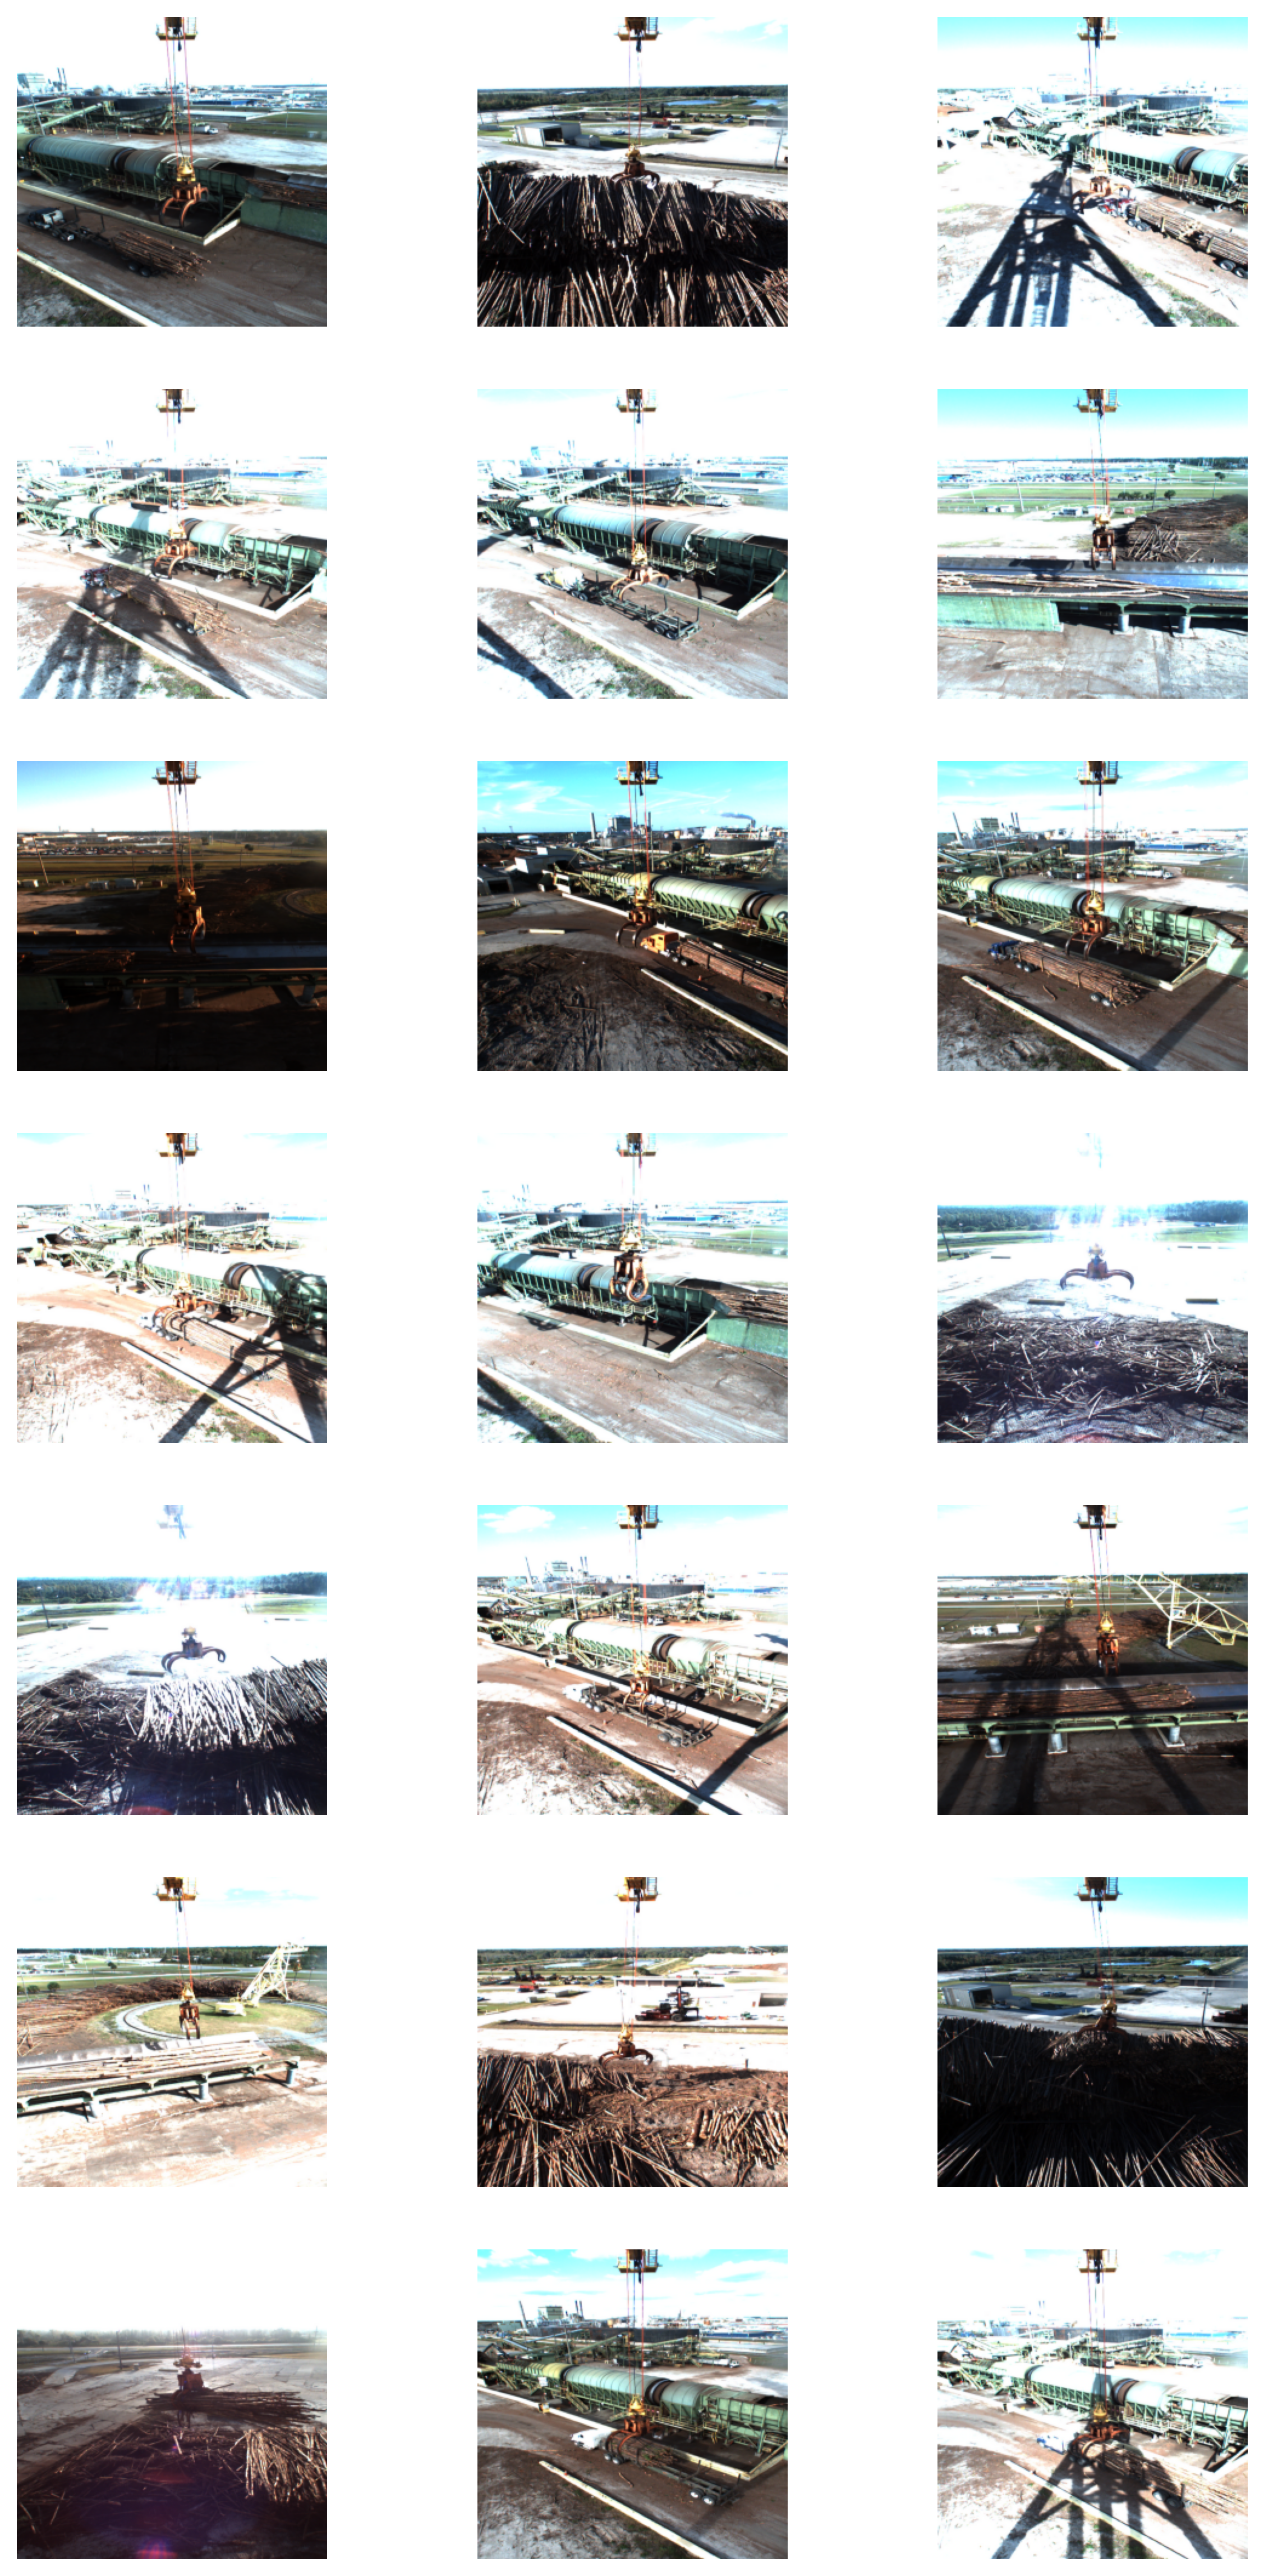
\includegraphics[width=0.7\textwidth, center]{bilder/Hauptteil/Transfer_Logs/LogsWrong.png}
	\caption{'Greifer beladen?' falsch vorhergesagt}
	\label{img:LogsFalschVorhergesagt}
	\end{figure}